\section{世界生成}
\label{sec:world}

\subsection{地形與 Chunk}

原本的作業規格使用 $[0,0,0]$ 到 $[50,0,50]$ 的平面。我將地板改成依 seed 生成的起伏地形，並切成邊長 16 m 的 chunk。
程式只保留機器人周圍半徑 12 個 chunk，移動時會釋放遠處區塊並生成新區塊，因此地形可以持續向外延伸（圖~\ref{fig:terrain}）。

地形高度由自行實作的 Perlin noise 與 fBm 產生，再依高度與環境參數決定地表顏色。
各 chunk 的內容由世界 seed 和座標決定，相同 seed 會得到相同結果。地形網格只在 chunk 第一次繪製時建立並快取，避免每幀重新取樣雜訊。

\subsection{障礙物}

每個 chunk 預先選定三個位置，分別嘗試放置方塊、球與圓柱；若位置位於水面或冰面則不生成。
方塊的長寬高與旋轉角度、球的半徑、圓柱的半徑與高度都由位置 seed 決定，尺寸上限為 2 m，顏色也使用同一 seed 產生。
障礙物底部貼齊當地地面，並和地形一樣轉成網格繪製，再套用第~\ref{sec:robot} 節依法向量計算的明暗效果。

\begin{figure}[htbp]
    \centering
    \begin{subfigure}[t]{.48\textwidth}
        \centering
        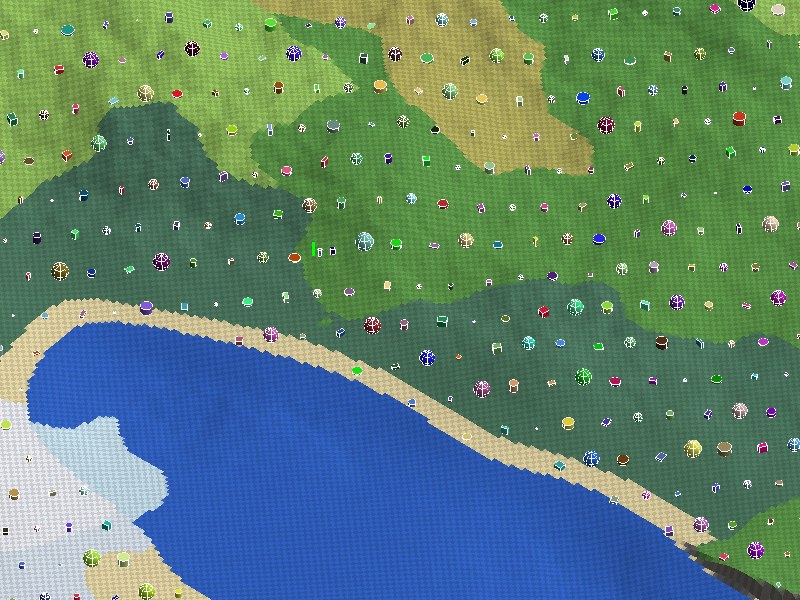
\includegraphics[width=\linewidth]{docs/figures/hw2/ch06_terrain.png}
        \caption{地形與生態系概觀}
    \end{subfigure}\hfill
    \begin{subfigure}[t]{.48\textwidth}
        \centering
        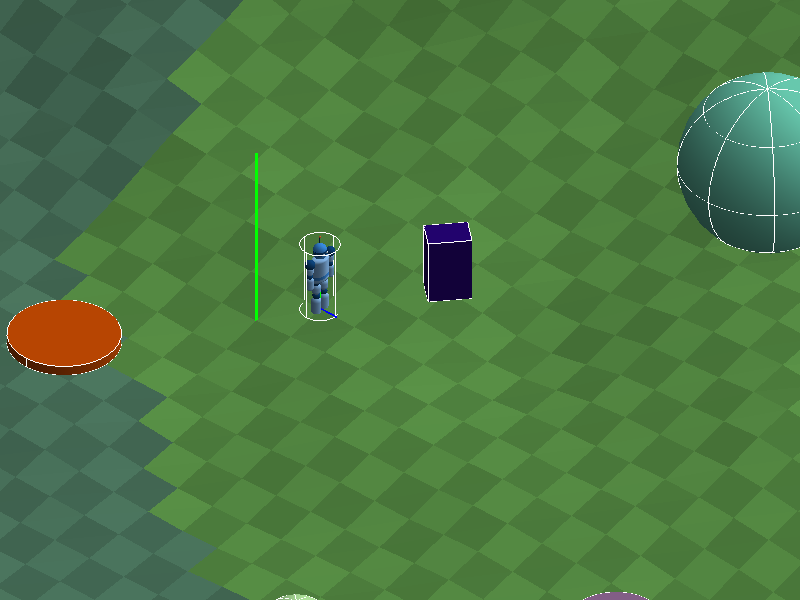
\includegraphics[width=\linewidth]{docs/figures/hw2/ch06_obstacles.png}
        \caption{方塊、球與圓柱障礙物}
    \end{subfigure}
    \caption{地形與障礙物}
    \label{fig:terrain}
\end{figure}
